\documentclass[12pt]{scrreprt}
\usepackage{listings}
\usepackage{underscore}
\usepackage{minted}
\usepackage[bookmarks=true]{hyperref}
\usepackage[utf8]{inputenc}
\usepackage[english]{babel}

\usepackage{tcolorbox}
\usepackage{hyperref}

\hypersetup{
    bookmarks=false,    % show bookmarks bar?
    pdftitle={FP PROJECT REPORT},    % title
    pdfauthor={Saptarishi Dhanuka},                     % author
    pdfsubject={TeX and LaTeX},                        % subject of the document
    pdfkeywords={TeX, LaTeX, graphics, images}, % list of keywords
    colorlinks=true,       % false: boxed links; true: colored links
    linkcolor=blue,       % color of internal links
    citecolor=black,       % color of links to bibliography
    filecolor=black,        % color of file links
    urlcolor=purple,        % color of external links
    linktoc=page            % only page is linked
}%
\def\myversion{1.0 }
\date{}
%\title
\usepackage{hyperref}
\newcommand{\ttt}[1]{\texttt{#1}}


\begin{document}




% ·        Title (with name, ID, supervisor, date)

% ·        Acknowledgement, if any

% ·        Table of Contents

% ·        Introduction

% ·        Background and Motivation

% ·        Literature Survey (state-of-the-art) – Gap Analysis, Research Questions etc.

% ·        Problem Statement / Objectives

% ·        Scope, Methodology, and Design – Architecture, HLD / LLD, if applicable

%  can have naive bayes in the methodology

% ·        Work Done – Implementations, Challenges, Mitigations, etc.

% ·        Results and Discussions

% ·        Conclusions (should highlight contribution)

% ·        Extensions and Future Work

% ·        References

 

% NOTES
% midterm feedback: First the specs should just contain the input output and not the method
% Req
% Spec
% Analysis
% Then architecture and design

% Explore llm for identifying interesting

% Explore pldi type thing

% First the project assumes html on the basis of tags. If not based on tags the
% the thing breaks. The specs shouldnt mention tagsoup and stuff. Should be independent of the method. But it should mention the limitations (?)

% In specs reduce the scope to assuming that using html and the tags are there using the parenthesisation problem. No don't do that in specs do that in the design  

% Original requirement doesn't mention that tags are there

% Just web page and get code and text

% Can u identify the code and the text without knowing the tags

% Mention in analysis

% Design shouldnt have the function details and stuff

% Architecture and design comes after analysing the the specs and requirements

% Specs in the presentation are wrong

% Get feedback from prof about what to do in report



% The specs are wrong. The specs should firstly mention the input output again after the requirments and mention it more technically like what separates the code from the text. It should NOT mention tagsoup or anything related to the method


% In the analysis of the specs then we can say that one way to tackle this problem is by assuming that the given web page is formatted in an correct HTML structure. Then we can extract the tags and solve the parenthesization problem for getting the code and the text out





% design flows from the specs so shouldn't have the function details and stuff directly 


\begin{flushright}
    \rule{16cm}{5pt}\vskip1cm
    \begin{bfseries}
        \Huge{FUNCTIONAL PROGRAMMING \\ CS-IS-2010-1 \\ FINAL PROJECT REPORT }\\
        \vspace{1.1cm}
        Topic: Haskell Scraper and Code-Text Separation\\
        \vspace{1.1cm}
        Name: Saptarishi Dhanuka\\
        \vspace{1.1cm}
        ID: 1020211525\\
        \vspace{1.1cm}
        Supervisor: Partha Pratim Das\\
        \vspace{1.1cm}
        Date: 13 May 2024\\
        \vspace{1.1cm}
        Ashoka University\\
    \end{bfseries}
\end{flushright}

\tableofcontents


\chapter{Acknowledgements}

I would like to thank Professor Das for taking this Independent Study Module and giving us the incentive to work on a software project in an unfamilar yet elegant language. I would also like to thank my fellow students as well as the teaching volunteers Gautam and Adwaiya for creating a wholesome learning environment. 


\chapter{Introduction}

%  cite stuff here cause references page is there and can't just say stuff in the air
%  maybe some motivation part here can go into the motivation section instead of the intro 

The large amounts of data in the form of interspersed code and natural language make it useful to extract knowledge from them in order to benefit various areas of software development. Examples like natural language comments accompanying code, stackoverflow questions and answers with code blocks, and developer emails containing discussions about code with reference to it are all important forms of such data. \\ 
\\ INSERT STUFF HERE!!!!!!!\\   
\\ For instance, extracting code and natural language separately from developer emails at a company can give key insights about how the company codebase has evolved and can help future developers access the code of emails directly. Separation of code and natural language is also helpful as training data for natural language and code completion models which can used the separated text and code to give better results. It creates a structured view of the code and textual data which can then further be used to create an organized view of the code and associated natural language. 


\chapter{Background and Motivation}


Consider the following image of an educational web page containing interspersed code and natural language:

\begin{figure}[h]
    \centering
    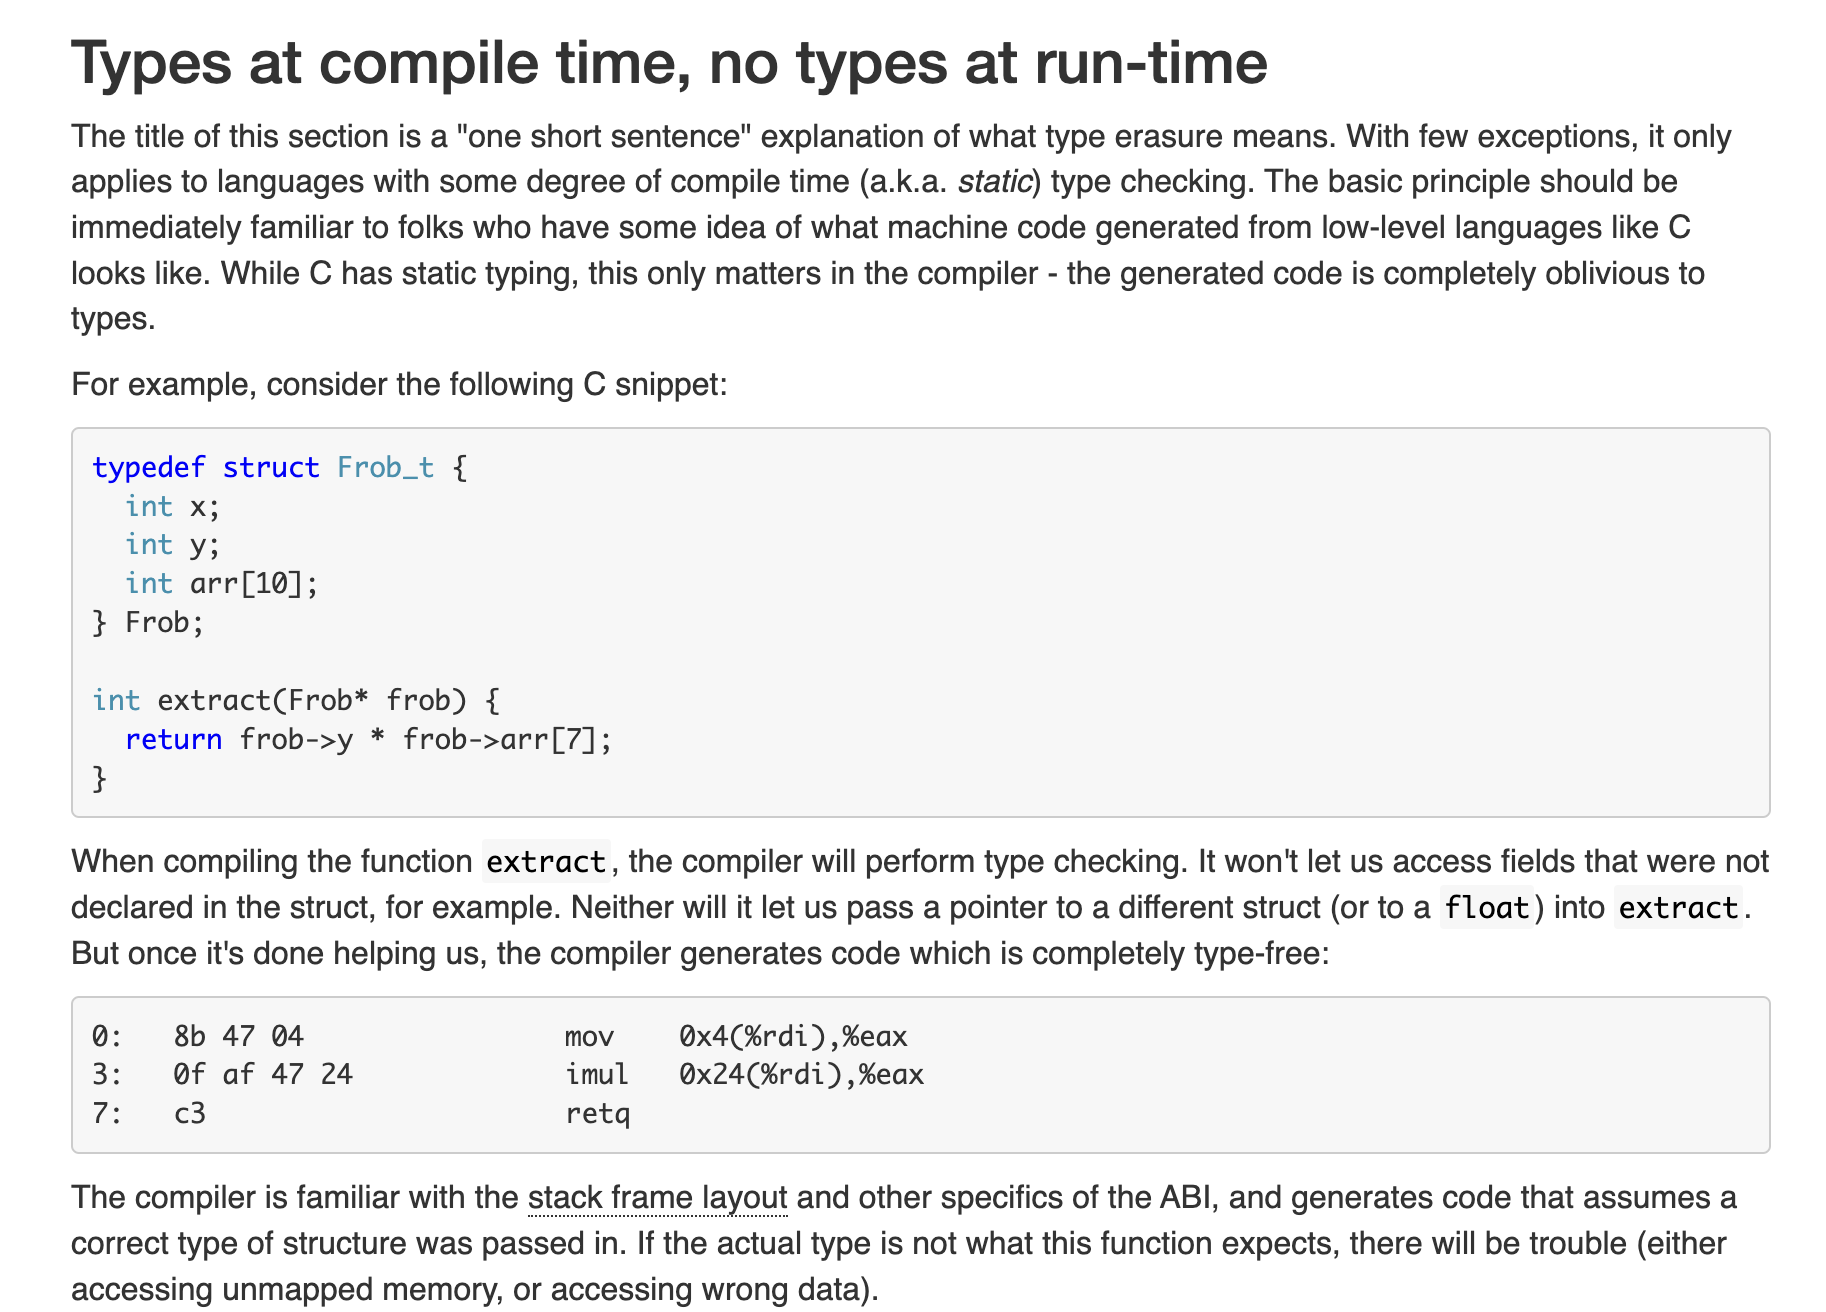
\includegraphics[width=0.7\textwidth]{figures/background-eg.png}
    \caption{Example of Code and Language Together}
    \label{fig:high-level-arch}
\end{figure}

Here it becomes useful to extract just the code or just the natural language separately if one just wants to run the code on their own machine or just wants the natural language descriptions for their notes or to get an overview of the idea being conveyed. Using HTML based separation of the text and code snippets, or trying to use regular expressions severely restricts the generalisability and accuracy of the system in extracting natural language and code separately.\\
\\ INSERT STUFF HERE!!!!!!!\\
\\ Towards this purpose, we will create a Naive Bayes classifier for classifying a particular line as natural language or code and creating two separate sections for all the natural language and all the code

\chapter{Literature Survey}

%  gap analysis and research questions ?????????????????

% basically that these guys did this and those guys did that and here's what I am gonna do and mention shortcomings and stuff later and say that did from scratch since haskell sde project






\chapter{Problem Statement and Objectives}
\begin{tcolorbox}[colback=white,colframe=gray,title={Assigned Project Statement}]
    Develop a scraper using Haskell to extract text and code snippets separately.
    \begin{enumerate}
        \item \textbf{Input}: Scrape the text and code snippets from the given text \href{https://eli.thegreenplace.net/2018/type-erasure-and-reification/}{source}
        \item \textbf{Output}: A Word document containing the text and \texttt{.txt} file containing the code.
        \item \textbf{Method}: Write the algorithm to scrape (you can use the \texttt{tagsoup} library) and all the input-output facilities using Haskell. Do not use any other language.
    \end{enumerate}
\end{tcolorbox}

% in the design section can give the basic structure of the HTML page

% \section{Problem Description}
% The given web page is made of text and code snippets, which we need to scrape and extract separately into a \texttt{.docx} file containing the text portions and a \texttt{.txt} file which has the code snippets. \\ For this, we need to fetch the given web page, parse and analyze it,so that we can effectively separate them into different documents.


\section{Requirements/Objectives}

\begin{enumerate}
    \item The user shall be able to give any text source as input.
    \item The scraper shall get all the code snippets of the source and write it into a Plaintext file.
    \item The scraper shall get all non-code text of the source and write it into a Word Document.
\end{enumerate}


\section{Specifications}

\begin{enumerate}
    \item The user will be able to enter a text source as input, whose code and non-code parts they wish to be separated.
    \item The scraper will parse the contents of the text and separate the code snippets from the rest of the text.
    \item The scraper will output a \texttt{.docx} file containing the textual content.
    \item The scraper will output a \ttt{.txt} file containing the code snippets.  
\end{enumerate}



% can mention that the scope is being restricted to with HTML stuff in the analysis
\section{Analysis}

\begin{enumerate}
    \item There are many ways of solving the problem both by syntactic and semantic approaches. Some semantic approaches are as follows:
        \begin{enumerate}
            \item Lexical and semantic analysis with the use of regular expressions
            \item Using a large language model to differentiate the code and the rest of the text 
            \item Using computer vision to attempt to read text like a human and identify text from the code
            \item Use the frequency of occurrence of different words in some sample data and use it to predict whether sections of unseen samples of text are natural language or source code. 
        \end{enumerate}
    \item Extracting the text and code snippets from a text source boils down to a classification task where we consider each new line as a line to be classified as natural language or code, and grouping them all into two separate sections depending on the class assigned to them.
    \item Hence we consider that the text source will consist of different newlines which need to be classified as language or code, without going into further granular details as to whether a particular word or phrase is code or text.
    %  we will take as input url but then just get the text from that url and nothing else. 
    

\end{enumerate}






\chapter{Scope and Methodology}

\section{Scope}
Following from the analysis, the system will classify text sources on a line level of granularity, hence it assumes that there will be some newline separation of different lines and the text source will not be completely unstructured. This is still a fairly broad scope since most text sources that have natural language and code interspersed in them have a newline-structure that make it easy to split them on a line-by-line basis for classification. 

% ADD STUFF HEREEEEEE!!!!

\section{Methodology}

The broad methodology is to train a Naive Bayes classifier on some custom training data consisting of natural language and source code, and then using the calculated probabilities to classify each line in the given text source as being code or natural language, and then separating them based on that. A brief overview of Naive Bayes is given below.
\subsection{Naive Bayes}







\chapter{Design and Architecture}
% need to put functions into Lib and main stuff in main
% mention directory structure here along with basic ideas of the functions and code what it's doing


% ·        Scope, Methodology, and Design – Architecture, HLD / LLD, if applicable


%  can have the design of the pipeline system from the text source to the two text files here. can do the results and stuff with the tables and the graphs later

\section{High-Level Architecture}

% insert image here
\begin{figure}[h]
    \centering
    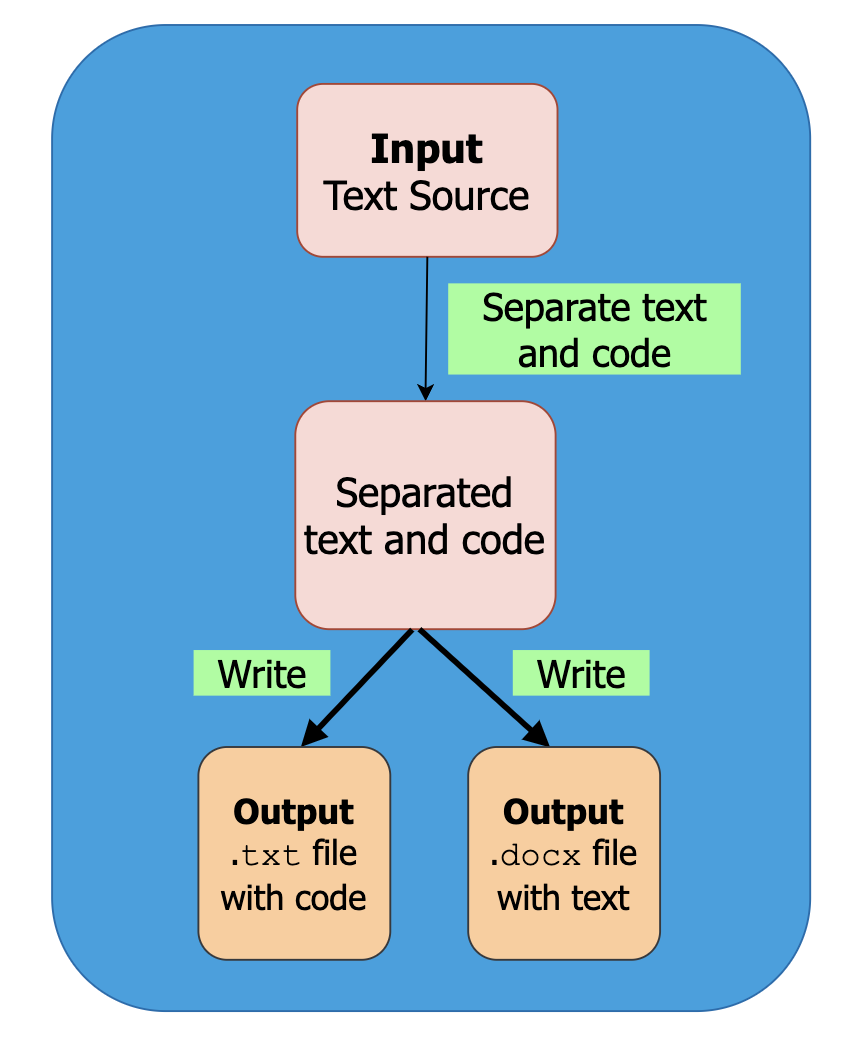
\includegraphics[width=0.6\textwidth]{figures/NB-high-arch.png}
    \caption{High-Level Architecture of Code-Text Separation Pipeline}
    \label{fig:high-level-arch}
\end{figure}


% change this cause it is not consistent with the design later need to make it so that the actual things like the tags and the text tags are in the boxes and the processes are on the arrows. 
The \textbf{high-level architecture} consists of the following:
\begin{enumerate}
    \item Get the contents of the text source
    % \item Parsing the response obtained from the HTTP libraries into Tags from the \texttt{tagsoup} library.
    % \item Separating the text from the code snippets using the descriptions of each Tag from the above Tags
    \item Separate the code snippets from the text.
    \item Writing the code snippets into a \texttt{.txt} file.
    \item Write the non-code textual content into a \texttt{.docx} file.
\end{enumerate}


\newpage 


\section{High-Level Design}


\begin{figure}[h]
    \centering
    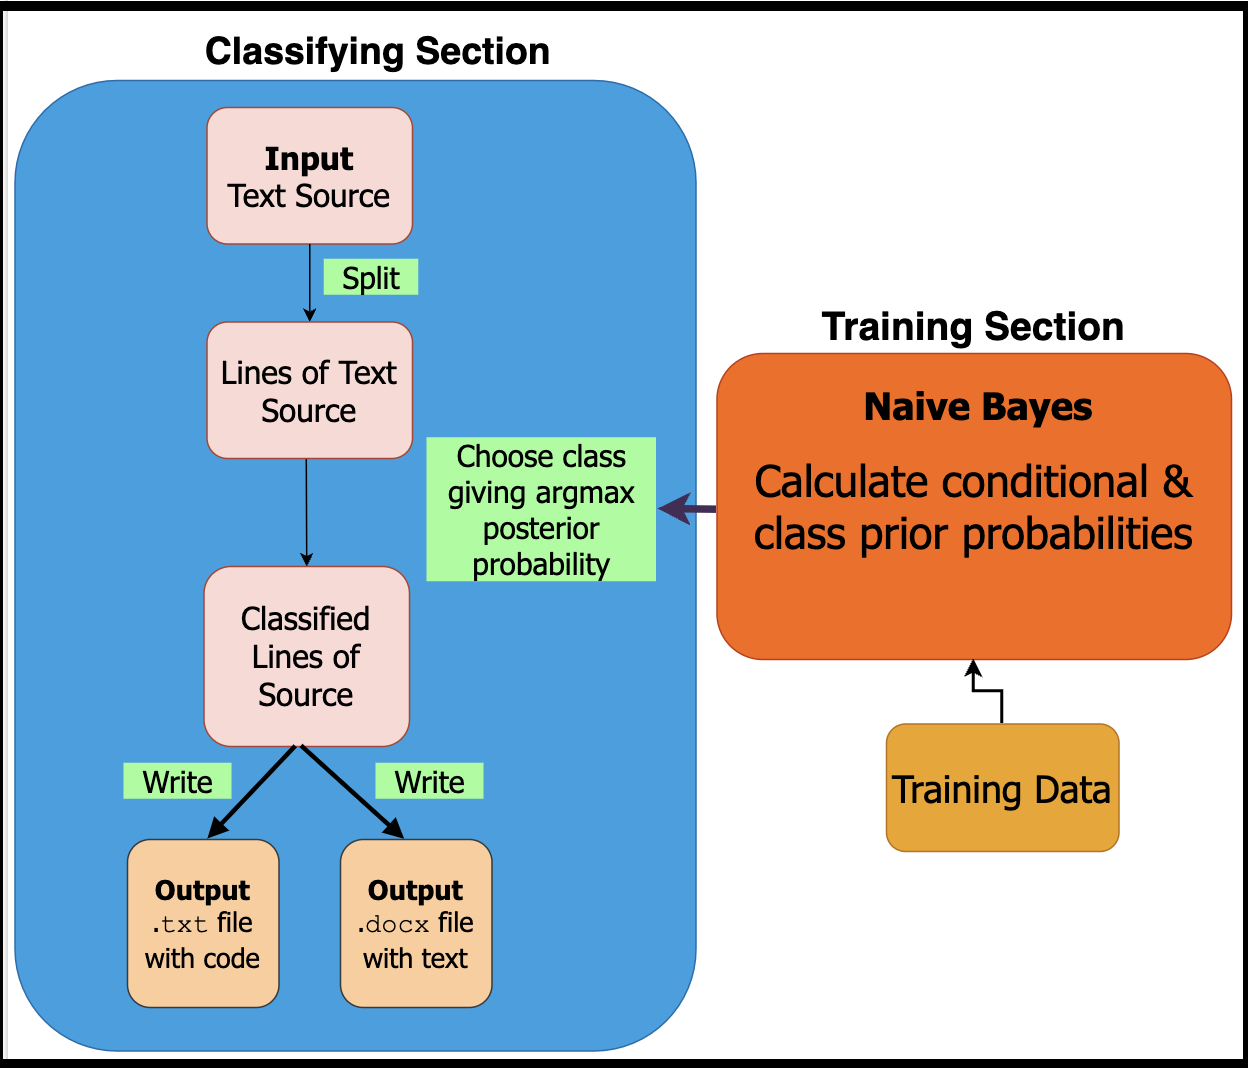
\includegraphics[width=1.0\textwidth]{figures/NB-high-design.png}
    \caption{High-Level Design of the Classifying Pipeline and Training Section}
    \label{fig:high-level-design}
\end{figure}

A more detailed description of the \textbf{high-level design} which implements the architecture broadly consists of two sections:
\begin{enumerate}
    \item \textbf{Training Section : }
    \begin{enumerate}
        \item Use natural language and source code training data already pre-classified in order to calculate the conditional probabilities and the class priors which make up the trained Naive Bayes Model.
    \end{enumerate}
    



    \item \textbf{Separatation Pipeline Section : }
    \begin{enumerate}
        \item Split the given text source into lines which will be considered as separate "documents" by the trained classificaton model.
        \item Classify each different line as source code or natural language text depending on which class has the higher posterior probability given that line
        \item Write the lines classified as source code into a \texttt{.txt} file
        \item Write the lines classified as natural language text into a \texttt{.docx} file
        % \item Execute an HTTPS request for fetching the HTML contents of the web page
        % % \item Parsing the url into a request
        % % \item Executing the request with the TLS manager
        % \item Get the body i.e. the HTML content from the response received after executing the request
        % \item Parse the HTML into a list of Tags according to the \texttt{tagsoup} library
        % \item Separate the Tags corresponding to the code from the Tags corresponding to the textual content. By inspecting the HTML, we can see that the code snippets are within \texttt{<pre>} tags, so we need to separate everything enclosed within these tags from the rest of the HTML content. We also remove images. 
        % \item Insert delimiters between each different code snippet for formatting purposes. 
        % % \item Convert the list of Tag Strings corresponding to the code and to the text each back into an HTML-formatted string, which we then convert into a \texttt{pandoc} document as intermediate representation
        % % \item Convert the pandocs into another intermediate string-like format which can then be written into the respective \texttt{.docx} and \texttt{.txt} files
        % \item Convert the Tags back to HTML
        % \item Write the code snippets to the \ttt{.txt} file
        % \item Write the non-code textual content to the \ttt{.docx} file
    \end{enumerate}

\end{enumerate}

The lower level implementation details are mentioned in the implementations section. 

%  should i specify network stuff here?

% I don't think I should mention the evaluation section since that doesn't affect the system. That part should go into results and anyway not much to talk about over there







\chapter{Implementation Details}
% this can give a broad overview of what the prototype can and cannot do. What the input and output of the prototype look like etc.


\section{File Structure}

% ?????????????????????????

% \begin{verbatim}
% scraper
% |-- app
% |   | -- Main.hs (main driver code)
% |-- src
% |   |-- Lib.hs (implementation of functions)
% |-- output_files
% |   | -- final_code.txt (delimited code snippets)
% |   | -- final_text.docx (textual content)


% \end{verbatim}




% in limitations can mention that need newline separated lines and we can't go beyond the granularity of a line since we did lines as documents based analysis



\section{Features and limitations}

The prototype correctly identifies the code and text portions of the web page and writes them into the \texttt{.txt} and \texttt{.docx} files as per the requirements and specifications. 

\subsubsection{Limitations}



\begin{enumerate}
            \item The prototype has not been robustly tested, verified for correctness or structured to handle errors. However, this can be developed while making the final system since the prototype is already relatively modular.
            \item Since the HTML structure of different web pages can vary, it is not necessary that this particular scraper will work for all web pages. It is designed specifically for the given page and may work for some other pages. But no generalisation can be made about the correctness of its text and code extraction for other pages.
            \item Moreover, it will not necessarily work for web pages with malformed HTML or different structure.
            \item It is not designed to be robust to design changes, which is in line with the \href{https://hackage.haskell.org/package/tagsoup-0.6/src/tagsoup.htm#:~:text=Rule%202%3A%0ADo%20not%20be%20robust%20to%20design%20changes%2C%20do%20not%20even%20consider%20the%20possibility%20when%20writing%20the%20code.}{rule} stated on the \texttt{tagsoup} library's documentation example, since the website's HTML can change in unpredictable ways. If the site's HTML structure changes, for instance if the code snippets change from being enclosed in \texttt{<pre>} tags to \texttt{<code>} tags, then the scraper will not be able to separate out the code from the text and extract them accurately.
            \item It clearly does not work with text sources that are not HTML formatted web pages.
\end{enumerate}


\newpage 
\section{Core Implementation Details}

Some important code and data features are shown that showcase the core implementation details of the project.


%  NEED TO HAVE A SECTION ABOUT THE DETAILS OF THE TRAINING DATA CAUSE THAT IS OBVIOUSLY ESSENTIAL TO THE SYSTEM

\subsection{Main.hs}

In-line with the design, architecture and choice of tools as mentioned above, the prototype obtains the HTML content of the url in line 2 and parses it into Tag Strings in line 3. Then we separate it into code tags and non-code textual tags in lines 4-6. Then we write the Tags to respective files in like 7-8.\\
\\ The core structure of the \texttt{Main.hs} file is
\begin{minted}{haskell}

    1. let url = "https://eli.thegreenplace.net/2018/type-erasure-and-reification/"
    2. response_html <- getHTML url
    3. let parsed_tags = parseTheTags response_html
    4. let separated_text_code = separateTextCode parsed_tags
    5. let preTags             = fst separated_text_code
    6. let nonPreTags          = snd separated_text_code
    7. writeToTxt preTags
    8. writeToDocx nonPreTags

\end{minted}

\subsection{Lib.hs}

\subsubsection{Imports and pragmas}

\begin{minted}[%
 breaklines,
 mathescape,
 linenos,
 numbersep=5pt,
 frame=single,
 numbersep=5pt,
 xleftmargin=0pt,
 ]{haskell}
{-# LANGUAGE OverloadedStrings #-}
import qualified Network.HTTP.Client as Client
import qualified Network.HTTP.Client.TLS as ClientTLS

import qualified Text.HTML.TagSoup as Soup
import Text.Pandoc

import qualified Data.Text.Conversions as TextConv
import qualified Data.Text as T
import qualified Data.Text.IO as TIO
import qualified Data.ByteString.Lazy as LBS
import qualified Data.ByteString.Lazy.Char8 as LBSC

\end{minted}

\subsubsection{getHTML}
\texttt{getHTML} takes the url as input and sets up a new TLS manager with \texttt{newTlsManager}, parses the url with \texttt{parseRequest} and then executes the request with \texttt{httpLbs}. \\ Then it gets the HTML content from the response using \texttt{responseBody}.

\begin{minted}[%
 breaklines,
 mathescape,
 linenos,
 numbersep=5pt,
 frame=single,
 numbersep=5pt,
 xleftmargin=0pt,
 ]{haskell}
getHTML :: String -> IO LBSC.ByteString
getHTML url = do
    mymanager <- ClientTLS.newTlsManager
    myrequest <- Client.parseRequest url
    response <- Client.httpLbs myrequest mymanager
    let response_html = Client.responseBody response
    return response_html
    
\end{minted}







\subsubsection{parseTheTags}
\texttt{parseTheTags} takes the HTML ByteString and parses it into a list of Tag Strings using \texttt{parseTags} from Tagsoup.

\begin{minted}[%
 breaklines,
 mathescape,
 linenos,
 numbersep=5pt,
 frame=single,
 numbersep=5pt,
 xleftmargin=0pt,
 ]{haskell}
parseTheTags :: LBSC.ByteString -> [Soup.Tag String]
parseTheTags response_html = (Soup.parseTags :: String -> [Soup.Tag String]) (LBSC.unpack response_html)
\end{minted}







\subsubsection{fillTrue}
\texttt{fillTrue} is a helper function that fills in True for every element enclosed within a matching pair of True statements corresponding to an opening and closing \texttt{<pre>} tags

\begin{minted}[%
 breaklines,
 mathescape,
 linenos,
 numbersep=5pt,
 frame=single,
 numbersep=5pt,
 xleftmargin=0pt,
 ]{haskell}
fillTrue :: [Bool] -> [Bool]
fillTrue [] = []
fillTrue [a] = [a]
fillTrue (False:False:xs) = False:fillTrue (False:xs)
fillTrue (False:True:xs) = False:fillTrue (True:xs)

-- fill True for elements after a <pre> tag starts
fillTrue (True:False:xs) = True:fillTrue (True:xs) 

-- seeing 2 consecutive Trues denotes end of <pre> tag, so skip them
fillTrue (True:True:xs) = True:True:fillTrue (xs) 
\end{minted}







\subsubsection{insertNewlines}
\texttt{insertNewLines} is a helper function that inserts a TagText for a delimiter before every closing \texttt{<pre>} tag for formatting purposes 

\begin{minted}[%
 breaklines,
 mathescape,
 linenos,
 numbersep=5pt,
 frame=single,
 numbersep=5pt,
 xleftmargin=0pt,
 ]{haskell}
insertNewlines :: [Soup.Tag String] -> [Soup.Tag String]
insertNewlines [] = []
insertNewlines (x:xs) = if (Soup.isTagCloseName "pre" x)
    then Soup.TagText "\n\n=======================\n\n":x:insertNewlines (xs)
    else x:insertNewlines (xs)
\end{minted}


\subsubsection{separateTextCode}
The idea of \texttt{separateTextCode} is as follows. Create a boolean list corresponding to every element of the list of Tag Strings. A boolean list element will be True if a Tag is a \texttt{<pre>} tag or within a \texttt{<pre>} tag. Then zip the boolean list with the original Tag list and get the Tags which have a correponding True value; this is the list of code tags. \\ Now mark elements to be true if the corresponding tags are \texttt{<img>} tags and create an overall boolean list which has false if the tag is not code and not an image. Extract the tags which have a false value; this is the list of non-code textual tags. \\ It essentially solves the parenthesization problem with the \ttt{<pre>} tags.

\begin{minted}[%
 breaklines,
 mathescape,
 linenos,
 numbersep=5pt,
 frame=single,
 numbersep=5pt,
 xleftmargin=0pt,
 ]{haskell}
separateTextCode :: [Soup.Tag String] -> ([Soup.Tag String], [Soup.Tag String])
separateTextCode parsed_tags =
    let bool_mapping_open = Prelude.map (Soup.isTagOpenName "pre") parsed_tags
        bool_mapping_close = Prelude.map (Soup.isTagCloseName "pre") parsed_tags

        -- do element-vise or of the two lists
        bool_mapping1 =  Prelude.zipWith (||) bool_mapping_open bool_mapping_close

        filled_true_pre = fillTrue bool_mapping1
        combined_pre = Prelude.zip filled_true_pre parsed_tags
        preTags = Prelude.map snd (Prelude.filter (fst) combined_pre)

        bool_mapping_img_open = Prelude.map (Soup.isTagOpenName "img") parsed_tags
        bool_mapping_img_close = Prelude.map (Soup.isTagCloseName "img") parsed_tags
        bool_mapping2 =  Prelude.zipWith (||) bool_mapping_img_open bool_mapping_img_close

        bool_mapping =  Prelude.zipWith (||) bool_mapping1 bool_mapping2

        filled_true = fillTrue bool_mapping
        -- zip parsed_tags list with the boolean list and Prelude.filter elements of the first list based on the second list to create tuple list
        combined = Prelude.zip filled_true parsed_tags
        -- get tags of tuples from combined where the boolean is false
        nonPreTags = Prelude.map snd (Prelude.filter (\(a,_) -> not a) combined)

    in (preTags, nonPreTags)


\end{minted}


\subsubsection{Writers to files}
\texttt{writeToTxt} takes the code Tags and renders them as an HTML formatted string after delimiting the snippets. Then the string is converted into the Text type, which is then fed into \texttt{readHtml} which converts it into an intermediate Pandoc format.\\ \texttt{writePlain} converts this pandoc into Text, which is finally written to the \texttt{.txt} file. \\
\\ \texttt{writeToDocx} takes the text Tags and renders them as an HTML formatted string. Then the string is converted into the Text type, which is then fed into \texttt{readHtml} which converts it into an intermediate Pandoc format.\\ \texttt{writeDocx} converts this pandoc into a ByteString, which is finally written to the \texttt{.txt} file. 

\begin{minted}[%
 breaklines,
 mathescape,
 linenos,
 numbersep=5pt,
 frame=single,
 numbersep=5pt,
 xleftmargin=0pt,
 ]{haskell}
writeToTxt :: [Soup.Tag String] -> IO ()
writeToTxt preTags = do
    let htmlPre = Soup.renderTags (insertNewlines preTags)
    pandocPre <- runIO $ readHtml def ( TextConv.convertText (htmlPre :: String ) :: T.Text )

    case pandocPre of
        Right x -> do
            y <- runIO $ writePlain def x
            case y of
                Right direct_pan_pre -> do
                    TIO.writeFile "output_files/final_code.txt" direct_pan_pre

                Left err -> Prelude.putStrLn $ "Error with pandoc writePlain: " ++ show err

        Left err -> Prelude.putStrLn $ "Error parsing pandoc for pre tags: " ++ show err
    
    putStrLn "Completed writing to txt"


writeToDocx :: [Soup.Tag String] -> IO ()
writeToDocx nonPreTags = do
    let htmlNonPre = Soup.renderTags nonPreTags
    pandocNoPre <- runIO $ readHtml def ( TextConv.convertText (htmlNonPre :: String ) :: T.Text )

    case pandocNoPre of
        Right x -> do
            y <- runIO $ writeDocx def x
            case y of
                Right direct_pan -> do
                    LBS.writeFile "output_files/final_text.docx" direct_pan

                Left err -> Prelude.putStrLn $ "Error with pandoc writeDocx: " ++ show err

        Left err -> Prelude.putStrLn $ "Error parsing pandoc for non pre tags: " ++ show err

    putStrLn "Completed writing to docx"

\end{minted}

\newpage


\section{Challenges and Mitigations}

Initially, I started the project by separating the code and text based on their HTML tags for the midterm project evaluation, but after feedback from Professor I decided to make the project much more generalized to any given text source instead of just HTML content due to the fragile nature of a system based on the latter. \\ I decided to implement the Naive Bayes algorithm from scratch due to it's ease of interpretability, simplicity, lightweightedness and surprisingly strong results. A brief outline of some challenges and mitigations are as follows:
\begin{enumerate}
    \item Before deciding on implementing Naive Bayes from scratch, I thought about using various methods like Hidden Markov Models and Support Vector Machines to create an ensemble learning method to classify text and code. However, library support in Haskell for these was not of good quality, hence I decided to implement Naive Bayes on my own.
    %  mention how good performance?
    \item In the implementation of Naive Bayes, another hurdle I faced was the inefficiency of the default \ttt{matrix} library in doing calculations with extremely large and sparse matrices, which was restricting me to training and testing sets of very small sizes, albeit with considerably good performance. So I looked for more efficient libraries and found the \ttt{hmatrix} library, which sped up computations by a large extent. Earlier a training and classification that took 2.5 minutes overall, now happened in 2.5 seconds. 
    \item The paucity of appropriate training data was also an issue. The few datasets that were relevant to the project, such as those containing source code along with some form of natural language (usually in the form of code comments) were all restricted to one language and were also immense for a classifier implemented from scratch without optimisations. Hence, I curated my own modestly size source code and natural language training data based on manual searching online
    \item The Haskell language was itself relatively challenging to get used to throughout the project due to it's difference from the imperative languages I am used to. But after learning lambda calculus and spending time with the language, it became easier to use and I could appreciate the elegance of functional programming more, even though I am still not as accustommed to this paradigm as I would like to be. 
\end{enumerate}




% maybe this can go after implementation details
\chapter{Tooling and Testing}

\section {Tools and Languages}
% tech stack
% need to be clear on cabal stack and haskell and stuff


\subsection{Languages}

Only Haskell was used for the project as mentioned in the problem statement

\subsection{Tools}

\begin{enumerate}
    \item The Glasgow Haskell Compiler (GHC) is used for compilation.
    \item \href{https://docs.haskellstack.org/en/stable/}{Stack} is used as the build tool. This manages installing project dependencies, building and running the project and testing the project.
    
    % say that hmatrix was used cause fastest
    \item \textbf{Libraries}:
    \begin{enumerate}
        \item 
        % \item \texttt{Network.HTTP.Client.TLS} was chosen for handling HTTPS connections in order to use the \texttt{newTlsManager} function
        % \item \texttt{Network.HTTP.Client} was chosen for parsing the url into a request, executing the request with the manager, and getting the body from the response. The functions used were \texttt{parseRequest, httpLbs, responseBody} respectively.
        % \item \texttt{Tagsoup} was used to parse the HTML into a list of Tag Strings, and then also to convert the separated Tag Strings back into an HTML-formatted string . It was also used in a helper function that inserted a delimiter between the code snippets. The functions used were \texttt{parseTags, isTagOpenName, isTagCloseName, renderTags}, along with the \texttt{TagText} constructor and \texttt{Tag} for \texttt{Tag String}.
        % \item \texttt{Pandoc} was used to read the HTML-formatted strings for both the code and the text into intermediate Pandoc representation. Then it was used to write the content into another intermediate string-like representation, which in turn was written into the final files with a standard library. The functions used were \texttt{readHtml, writePlain, writeDocx, runIO}.
        % \item \texttt{Data.ByteString.Lazy.Char8} was used to convert the ByteString obtained from the response body into a string for further processing. The function used was \texttt{unpack}
        % \item \texttt{Data.ByteString.Lazy} was used to write the ByteString obtained from the \texttt{writeDocx} function from \texttt{pandoc}, into the final \texttt{.docx} file. The function used was \texttt{writeFile}
        % \item \texttt{Data.Text.Conversions} was used to convert the separated HTML strings into the \texttt{Text} type defined under \texttt{Data.Text}, so that it could be converted into intermediate pandoc representation by \texttt{readHtml}. The function used was \texttt{convertText}.
        % \item \texttt{Data.Text} was used in order to use the \texttt{Text} type
        % \item \texttt{Data.Text.IO} was used to write the Text obtained from the \texttt{writePlain} function from \texttt{pandoc}, into the final \texttt{.txt} file. The function used was \texttt{writeFile}
        % \item The standard \texttt{Prelude} was used for various operations.
    \end{enumerate} 
\end{enumerate}






\section{Testing}
% test individual functions 
% for the midterm eval at the end if have time (need to) then can write one big test 

% \section{Tools to be used for Testing}



\subsection{Test Suite Outline}

\begin{enumerate}
    \item \textbf{Unit Testing : } The following functions can be tested 
    \begin{enumerate}
        \item \texttt{getHTML : }
        \begin{enumerate}
            \item Test if the function returns the correct HTML for various URLs by using sample inputs and outputs.
            \item Test if the function gracefully handles invalid URLs with error handling.
            \item Test if the function handles network errors and HTTPS errors with error handling.
        \end{enumerate}

        \item \texttt{parseTheTags : }
        \begin{enumerate}
            \item Test if the function returns the correct list of Tag Strings for various HTML content.
            \item Test if the function handles malformed HTML and erroneous inputs with error handling.
        \end{enumerate}

        \item \texttt{fillTrue : }
        \begin{enumerate}
            \item Test if the function correctly fills in True values for all elements within any two matching pair of True values corresponding to \texttt{<pre>} tags.
            \item Test if the function handles edge cases with empty lists or single element lists.
        \end{enumerate}

        \item \texttt{insertNewLines : }
        \begin{enumerate}
            \item Test if the function correctly adds the delimiter before every closing \texttt{<pre>} tag.
            \item Test if the function handles cases where there are no \texttt{<pre>} tags, or the Tag String is malformed 
        \end{enumerate}

        \item \texttt{separateTextCode : }
        \begin{enumerate}
            \item Test if the function correctly returns a tuple of two lists where one list has the Tag Strings corresponding to all the content enclosed within \texttt{<pre>} tags, and that the other list has all the other elements, excluding images.
            \item Test edge cases of no \texttt{<pre>} tags, nested \texttt{<pre>} tags
        \end{enumerate}

        \item \texttt{writeToTxt : }
        While File I/O cannot be unit-tested in the traditional sense, we can still manually test the file outputs.
        \begin{enumerate}
            \item Test if the function correctly writes the content of the input Tag String with delimters to the \texttt{.txt} file using sample input output
        \end{enumerate}

        \item \texttt{writeToDocx : }
        While File I/O cannot be unit-tested in the traditional sense, we can still manually test the file outputs.
        \begin{enumerate}
            \item Test if the function correctly writes the content of the input Tag String to the \texttt{.docx} file using sample input output
        \end{enumerate}

    \end{enumerate}
    \item \textbf{Performance Testing : } 
    \begin{enumerate}
        \item Test the time taken for the full system to execute from start to finish
        \item Test the resource consumption of the system
    \end{enumerate}
    \item \textbf{Functional Testing : } \\ Test whether the program meets the requirements by using sample input URLs and sample output files
\end{enumerate}


\subsection{Test Report}






\chapter{Plan for Completion}
% will test. will do error handling. formal verification and validation stuff and maybe make more robust for other urls also idk. Getting better performance


\begin{itemize}
    \item Implement error handling gracefully wherever possible so that no unhandled errors can occur.
    \item Implement the test suite
    \item Attempt to make the scraper more generalized so that it can work with other websites and other HTML structures.
    \item Document the code well
    \item Explore methods of separating the code from the non-code textual content that are independent of HTML structure. Such methods were mentioned in the analysis and implementation of these methods will make the scraper more generalizable. 
\end{itemize}


\chapter{Results and Discussions}

The classifier was run on various natural language and source code files and the results were collected. Metrics like precison and recall with respect to code and language, along with the F-measure were calculated. We found that even with the highlight simplistic design and the strong Naive Bayes assumptions, the classifier could perform surprisingly well in classifying lines as code or natural language.

%  graphs and stuff


%  pie charts and stuff


% tables and stuff 


\chapter{Conclusions}
%  should highlight contributions
%  lightweight text and code separation in functional programming language so it can be easily verified or smth
% it's also very interpretable and linear time complexity stuff



\chapter{Extensions and Future Work}



\chapter{References}















\end{document}